\section{Predicción de saltos}

\begin{frame}[t]{Bifurcaciones y tiempo de ejecución}
\begin{itemize}
  \item Cada bifurcación condicional está \textmark{fuertemente sesgada}.
    \begin{itemize}
      \item O se toma la mayoría de las veces,
      \item O no se toma la mayoría de las veces.
    \end{itemize}

  \mode<presentation>{\vfill\pause}
  \item \textgood{Predicción basada en perfil de ejecución}:
    \begin{itemize}
      \item Se ejecuta una vez para recoger estadísticas.
      \item Se utiliza la información recogida para modificar el código y aprovechar la información.
    \end{itemize}
\end{itemize}
\end{frame}

\begin{frame}[t]{Predicciones con perfil de ejecución}
\begin{itemize}
  \item SPEC92: Frecuencia de bifurcaciones 3\% a 24\%
  \item \textgood{Coma flotante}:
    \begin{itemize}
      \item \textgood{Fallo de predicción}. 
        \begin{itemize}
          \item \textmark{Media}: 9\%. 
          \item \textmark{Desviación estándar}: 4\%.
        \end{itemize}
    \end{itemize}
  \item \textgood{Enteros}:
    \begin{itemize}
      \item \textgood{Fallo de predicción}. 
        \begin{itemize}
          \item \textmark{Media}: 15\%. 
          \item \textmark{Desviación estándar}: 5\%.
        \end{itemize}
    \end{itemize}
\end{itemize}
\end{frame}

\begin{frame}[t]{Predicciones con perfil de ejecución}
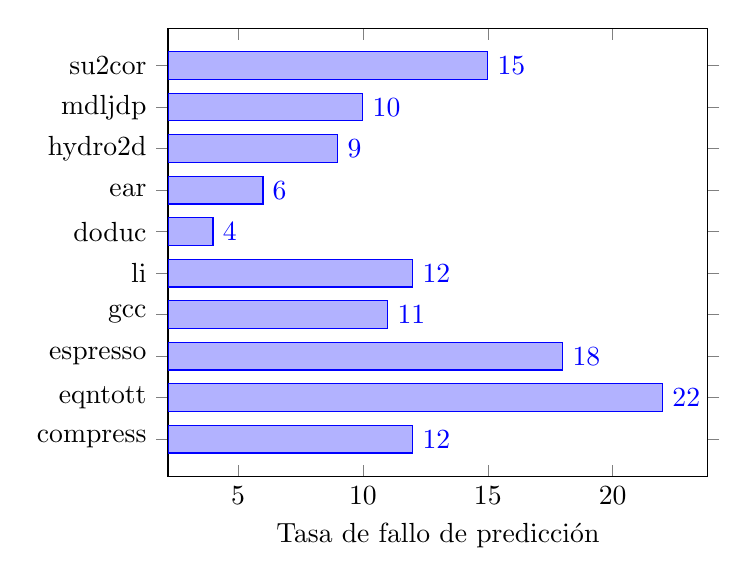
\begin{tikzpicture}
  \begin{axis}[
    xbar,
    xlabel={Tasa de fallo de predicción},
    symbolic y coords={compress,eqntott,espresso,gcc,li,doduc,ear,hydro2d,mdljdp,su2cor},
    ytick=data,
    nodes near coords, nodes near coords align={horizontal},
    ]
    \addplot coordinates {
(12,compress) 
(22,eqntott)
(18,espresso)
(11,gcc)
(12,li)
(4,doduc)
(6,ear)
(9,hydro2d)
(10,mdljdp)
(15,su2cor)
};
  \end{axis}
\end{tikzpicture}
\end{frame}

\begin{frame}[t]{Predicción dinámica: BHT}
\begin{itemize}
  \item Tabla histórica de saltos (Branch History Table)
    \begin{itemize}
      \item \textmark{Índice}: Bits menos significativos de dirección (PC).
      \item \textmark{Valor}: 1 bit (salto tomado o no la última vez).
    \end{itemize}
  \item \textgood{Efectos}:
    \begin{itemize}
      \item Se desconoce si la predicción es correcta.
        \begin{itemize}
          \item Podría venir de otra instrucción situada en una dirección
                diferente con los mismos bits menos significativos.
        \end{itemize}
        \item Número de bits menos significativos implica tamaño de búfer.
          \begin{itemize}
            \item 10 bits $\Rightarrow$ 1024 entradas.
          \end{itemize}
        \item Si la predicción falla se invierte bit.
        \item \textbad{Desventaja}: Bifurcación de bucle falla dos veces.
          \begin{itemize}
            \item Primera y última iteración.
          \end{itemize}
    \end{itemize}
\end{itemize}
\end{frame}

\begin{frame}[t]{Predicción dinámica: BHT}
\begin{itemize}
  \item Tabla histórica de saltos (Branch History Table)
    \begin{itemize}
      \item \textmark{Índice}: Bits menos significativos de dirección (PC).
      \item \textmark{Valor}: 1 bit (salto tomado o no la última vez).
        \begin{itemize}
          \item \textgood{00} y \textgood{01}: Predecir a no tomado.
          \item \textgood{10} y \textgood{11}: Predecir a tomado.
        \end{itemize}
    \end{itemize}
\end{itemize}
\makebox[\textwidth][c]{
\input{es/m4-02-ilp/bht-statediag.tkz}
}
\begin{itemize}
  \item \textgood{Mejoras}: Uso de más bits para mejorar la precisión.
\end{itemize}
\end{frame}

\begin{frame}[t,shrink=10]{BHT: Precisión}
\begin{itemize}
  \item Fallos de predicción:
    \begin{itemize}
      \item Predicción errónea para el salto.
      \item Historia de otro salto en la entrada de la tabla.
    \end{itemize}
\item Resultados BHT de 2 bits y 4K entradas:
\end{itemize}
\begin{tikzpicture}
  \begin{axis}[
    xbar,
    width=\textwidth, height=0.7\textheight,
    xlabel={Tasa de fallo de predicción},
    symbolic y coords={li,eqntott,espresso,gcc,fpppp,spice,doduc,tomcatv,matrix300,nasa7},
    ytick=data,
    nodes near coords, nodes near coords align={horizontal},
    ]
    \addplot coordinates {
(10,li)
(18,eqntott)
(5,espresso)
(12,gcc)
(9,fpppp)
(9,spice)
(5,doduc)
(1,tomcatv)
(0,matrix300)
(1,nasa7)
};
  \end{axis}
\end{tikzpicture}
\end{frame}

\begin{frame}[t]{Predicción dinámica de bifurcación}
\begin{itemize}
  \item ¿Por qué funciona la predicción de saltos?
    \begin{itemize}
      \item El algoritmo presenta regularidades.
      \item Las estructuras de datos presenta regularidades.
    \end{itemize}

  \mode<presentation>{\vfill}
  \item ¿Es mejor la predicción dinámica que la predicción estática?
    \begin{itemize}
      \item Parecer serlo.
      \item Hay un pequeño número de bifurcaciones importantes en programas con comportamiento dinámico.
    \end{itemize}
\end{itemize}
\end{frame}
